\subsection{Reporting and next steps}
\label{sec:reporting}

\begin{table}[!h]
    \centering
    % set up banded rows for the agenda and add lines to the columns
    \arrayrulecolor{Task32Blue2!15}
    \rowcolors{2}{Task32Blue2!5}{white}
    \begin{tabular}{@{}
        |p{0.175\columnwidth-2\tabcolsep}
        |p{0.825\columnwidth-2\tabcolsep}
        |@{}}
    \rowcolor{Task32Blue2} \textbf{Time} & \textbf{Activity} \\    
    16:00 & Reporting and next steps \\
    16:55 & Break
    \end{tabular}
    \label{tab:day4-results-agenda}
\end{table}

43 participants joined us to hear about the outcomes from the working groups.

Each group was allocated 1 slide and 3 minutes to present their work. Each group appointed a rapporteur to present their work.

Following are the notes from each group including the summary slide that they prepared. The slides have been reproduced without editing.

\subsubsection{Forecasting}

\emph{Rapporteur: Ines Würth}

This is a topic with lots of open questions, but there's not much public research in this area at the moment. Task 32 remains a great place to share ideas. %More information about the discussion in this group is available in the \href{https://docs.google.com/document/d/1Yq2JyWJAEZVAJE9te4FJ-57OpXdxNRHWhks88l2YJcI/edit?usp=sharing}{working group's notes}.

\begin{taskactions}
\textbf{Task 32 action}: we'll store those open questions in a public space and make them available for others to build on.
\end{taskactions}

\subsubsection{Wind lidar for wind energy applications in cold climate}

\emph{Rapporteur: Nicolas Jolin}

See the presentation from Day 2 for more information about this working group. Studies are ongoing. Please get in contact with Nicolas Jolin if you are interested.

\begin{taskactions}
\textbf{Task 32 action}: Task 32 will continue to support this working group.
\end{taskactions}

\subsubsection{A world without cups}

\emph{Rapporteur: Mads Sorensen, Remi Gandoin}

\begin{itemize}
\item These were more philosophical discussions. But it's important to think about philsophy when looking into the future.
\item An entire industry needs to be changed!
\item the laser technology and the great progress it lead to in physics;
\item going beyond the \enquote{lidars don't give me TI} concerns and approach by questioning/better understanding what these TI values are used for (typically to evaluate the IEC turbulence class). In effect, in the IEC framework, the input flow models that are used for the load simulations are really \enquote{toy} models of the atmosphere (i.e., steady-state over 10 minutes, power law shear, and Kaimal neutral form spectra with pre-defined length scales). Despite the potential of wind lidar, we are missing practical examples of situations where LiDARs lead to better siting/WTG choice than cups.
\end{itemize}

\begin{taskactions}
\textbf{Task 32 action}: Task 32 will continue to explore this question. We may identify a work case that is not well-served by cup anemometers and the current approach to wind characterisation, and investigate how to leverage wind lidar instead.
\end{taskactions}

\subsubsection{Collaboration on wind lidar hardware and software}

\emph{Rapporteur: Francisco Costa}

There's a lot of work going on in this area. The major challenge is to coordinate activities and tools, and enable them to work together (\fref{fig:day3-collaboration-hardware-software}).

% \begin{figure*}[p]
% \centering
% \fbox{
% 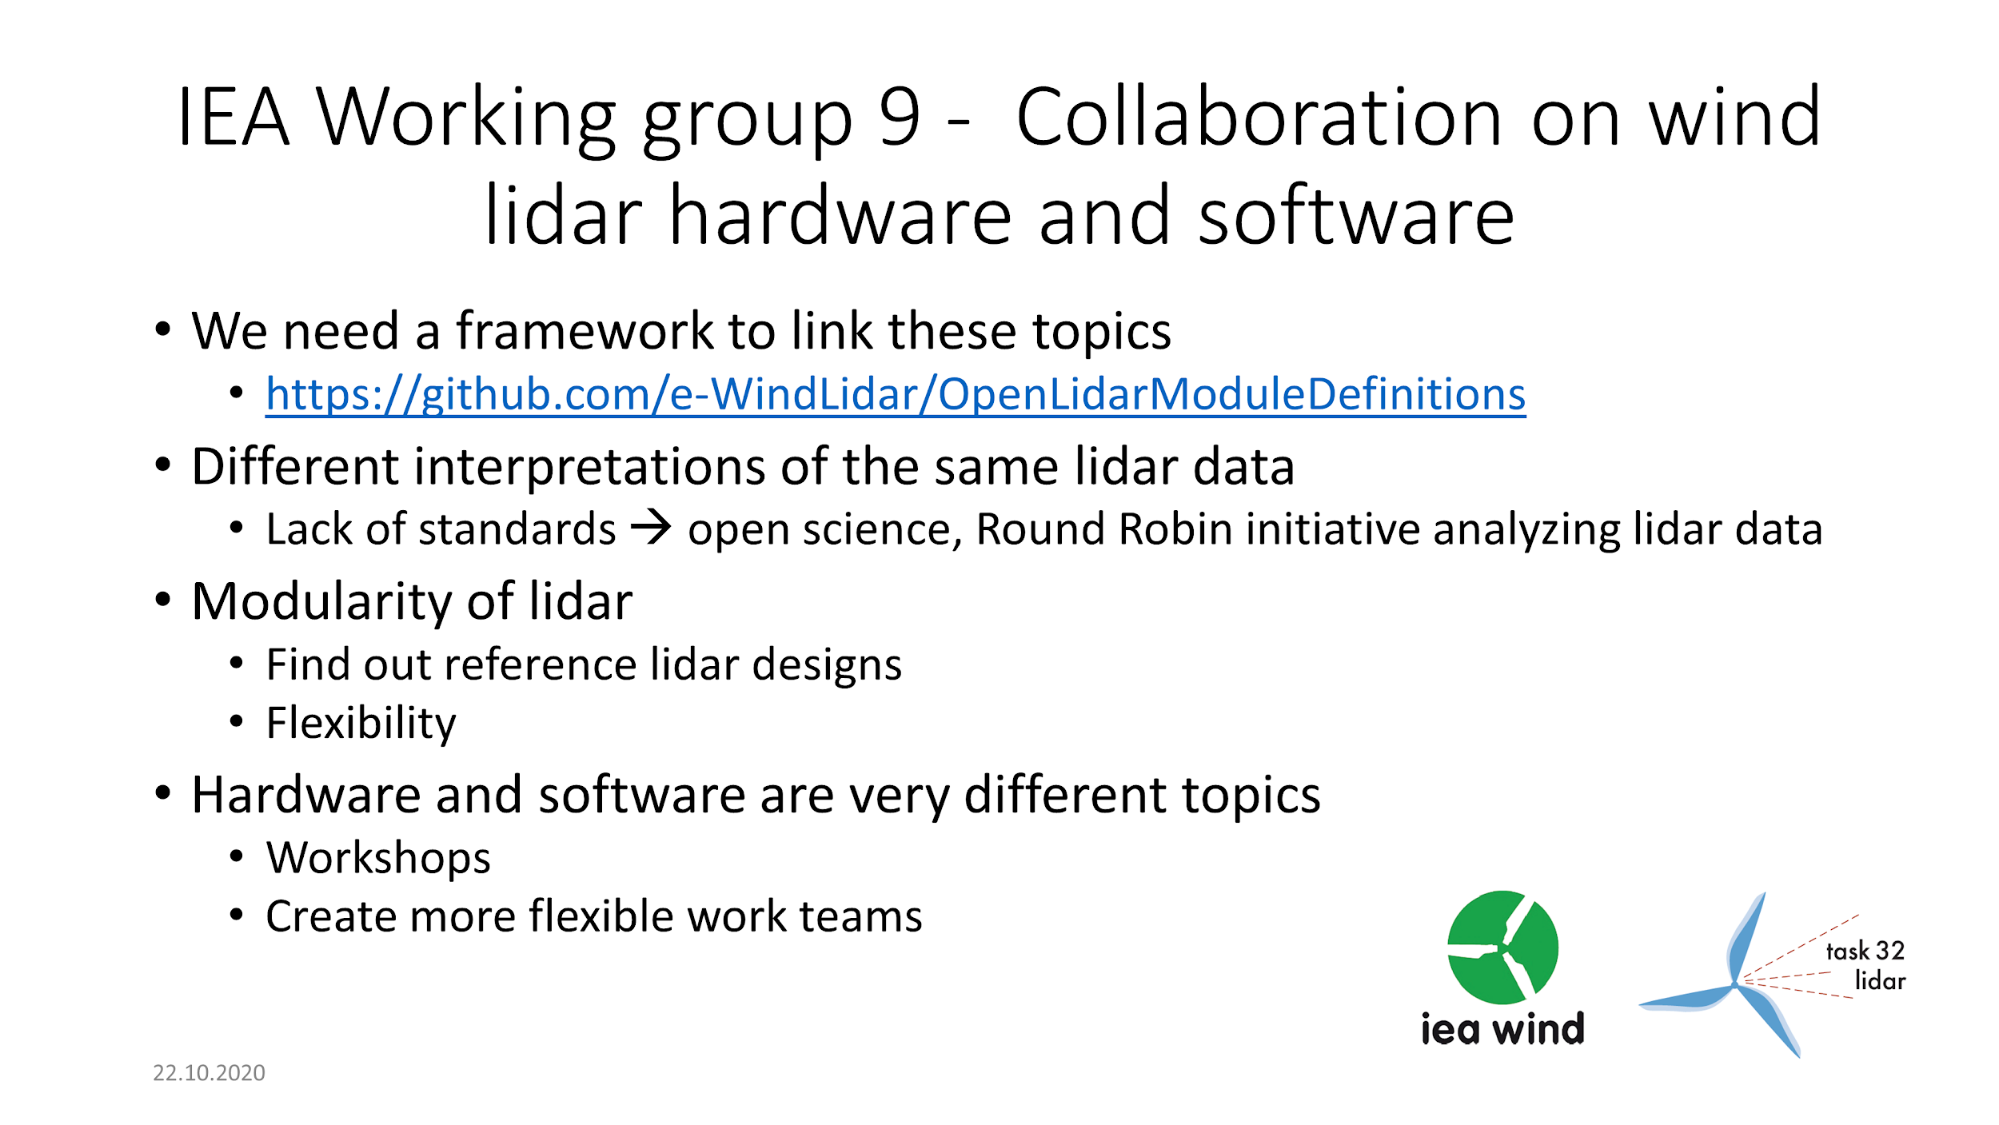
\includegraphics[width=0.85\textwidth]{figures/day3-collaboration-hardware-software.png}
% }
% \caption{Collaboration on wind lidar hardware and software}
% \label{fig:day3-collaboration-hardware-software}
% \end{figure*}
\begin{taskactions}
\textbf{Task 32 action}: we'll update the \href{https://github.com/IEA-Wind-Task-32/wind-lidar-glossary}{Task 32 Glossary} to include a generic lidar design approach that is aligned with the open lidar modular concept \cite{clifton_2019_openlidar}. This glossary can be used to define classes for lidars, like \emph{optics.telescope.aperture} which could help with defining inputs for simulations, etc. We'll also create reference designs using this structure.
\end{taskactions}

\subsubsection{Turbulence intensity derived from wind lidar}

\emph{Rapporteur: Reesa Dexter}

This has been a recurrent theme through the General Meeting. There are opportunities to go beyond current approaches to just mirror conventional met masts (\fref{fig:day3-Ti-group}). A workshop bringing industry and academia together would be a good next step.

% \begin{figure*}[p]
%     \centering
%     \fbox{
%     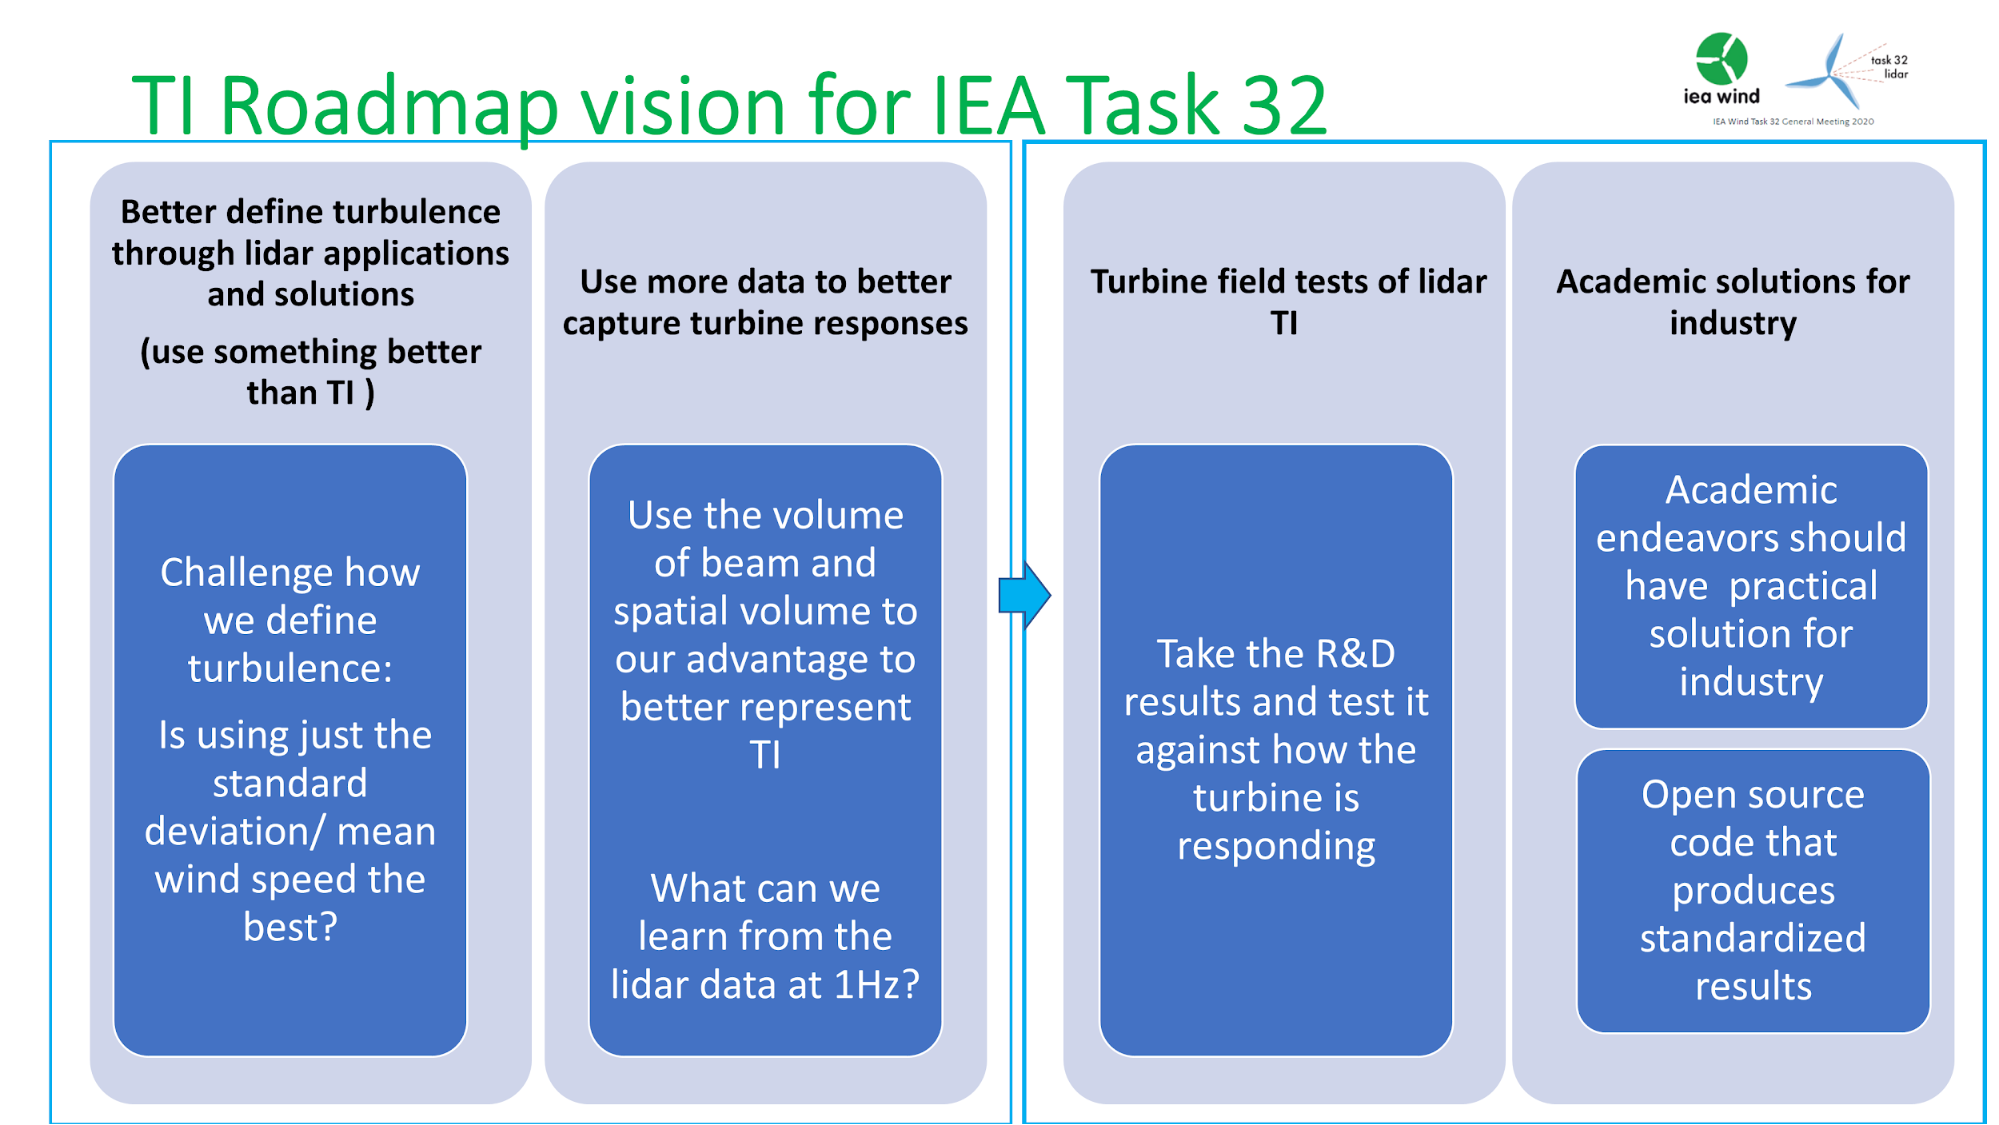
\includegraphics[width=0.85\textwidth]{figures/day3-Ti-group.png}
%     }
%     \caption{A lidar-derived turbulence data roadmap vision for Task 32 }
%     \label{fig:day3-Ti-group}
% \end{figure*}

\begin{taskactions}
\textbf{Task 32 action}: we'll include the suggested next steps in our roadmap and start to plan events for 2021 and beyond. We'll also coordinate with CFARS.
\end{taskactions}

\subsubsection{Wind lidar in complex terrain}

\emph{Rapporteur: Alexander St\"okl}

There continues to be a lot of interest in the potential to use wind lidar in complex terrain. This means we need tools to do it reliably and predictably, and we need to know when we hit the limits of our capabilities (\fref{fig:day3-complex-terrain}). There's an active Task 32 working group in this area, led by Alexander (see \sref{sec:news-complex-terrain-group}.)

% \begin{figure*}[p]
%     \centering
%     \fbox{
%     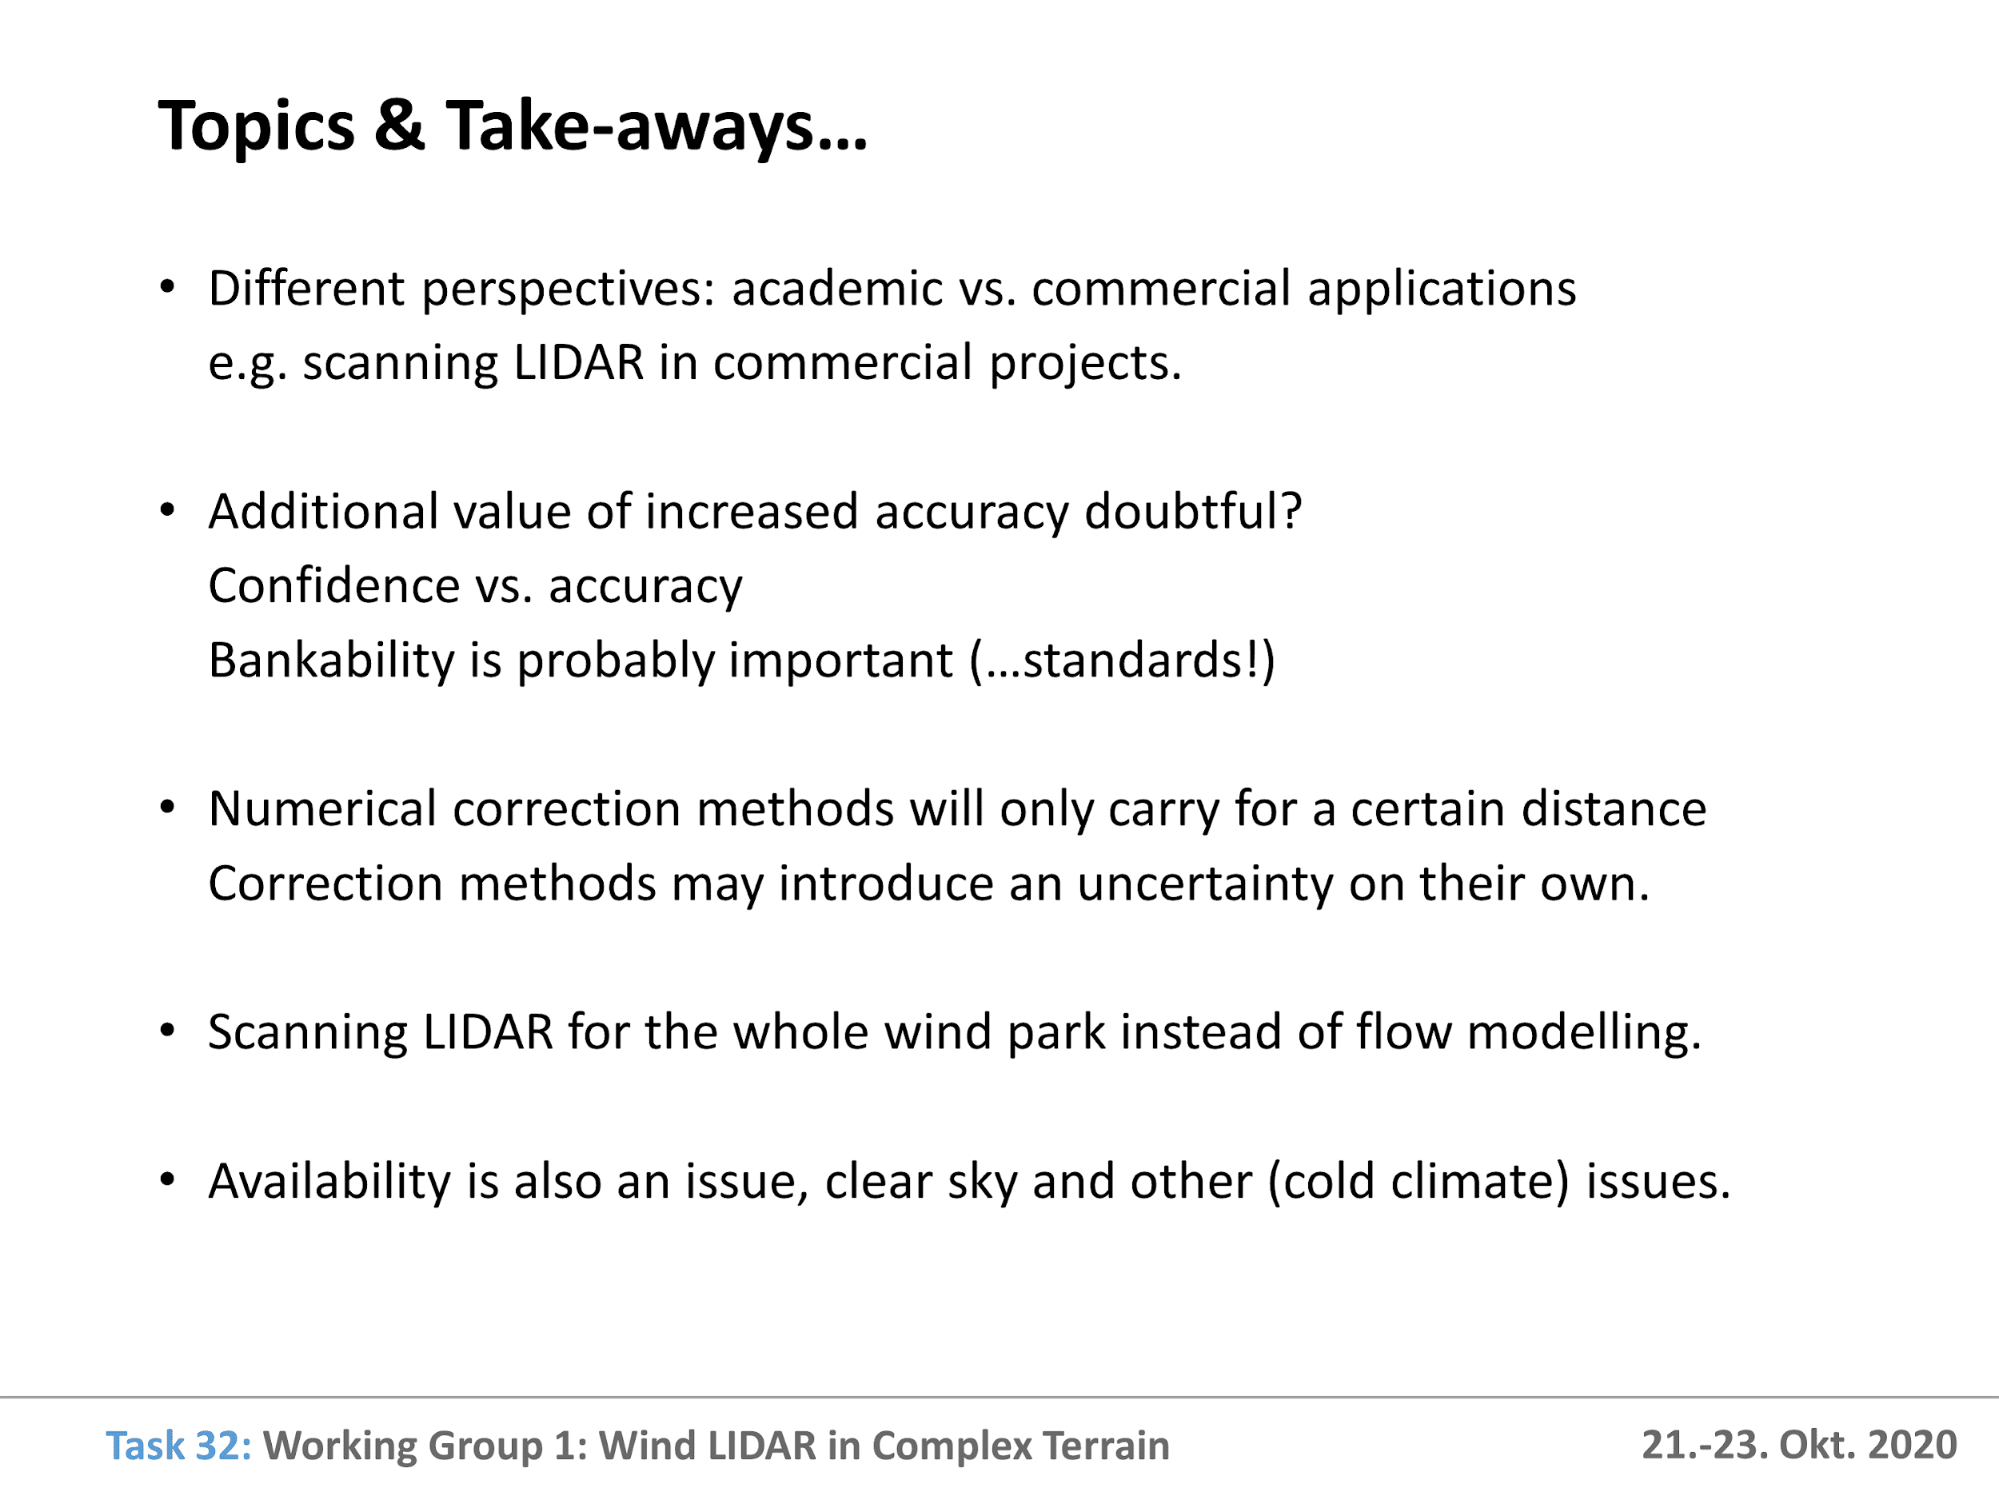
\includegraphics[width=0.85\textwidth]{figures/day3-complex-terrain.png}
%     }
%     \caption{Topics and take-aways from the complex terrain working session}
%     \label{fig:day3-complex-terrain}
% \end{figure*}

\begin{taskactions}
\textbf{Task 32 action} : Task 32 will continue to support this working
group.
\end{taskactions}

\subsubsection{Floating lidar}

\emph{Rapporteur: Julia Gottschall, IWES Fraunhofer}

The majority of actions around floating lidar are taking place through the IEC, and it is not needed at this time to have parallel activities through Task 32 as many stakeholders are already taking part in the IEC process. However, not all are involved and there is a need to make sure that the Task 32 community and IEC maintain alignment. The suggestion is therefore a third workshop in the second half of 2021 to align (\fref{fig:day3-floating-lidar}).

% \begin{figure*}[p]
%     \centering
%     \fbox{
%     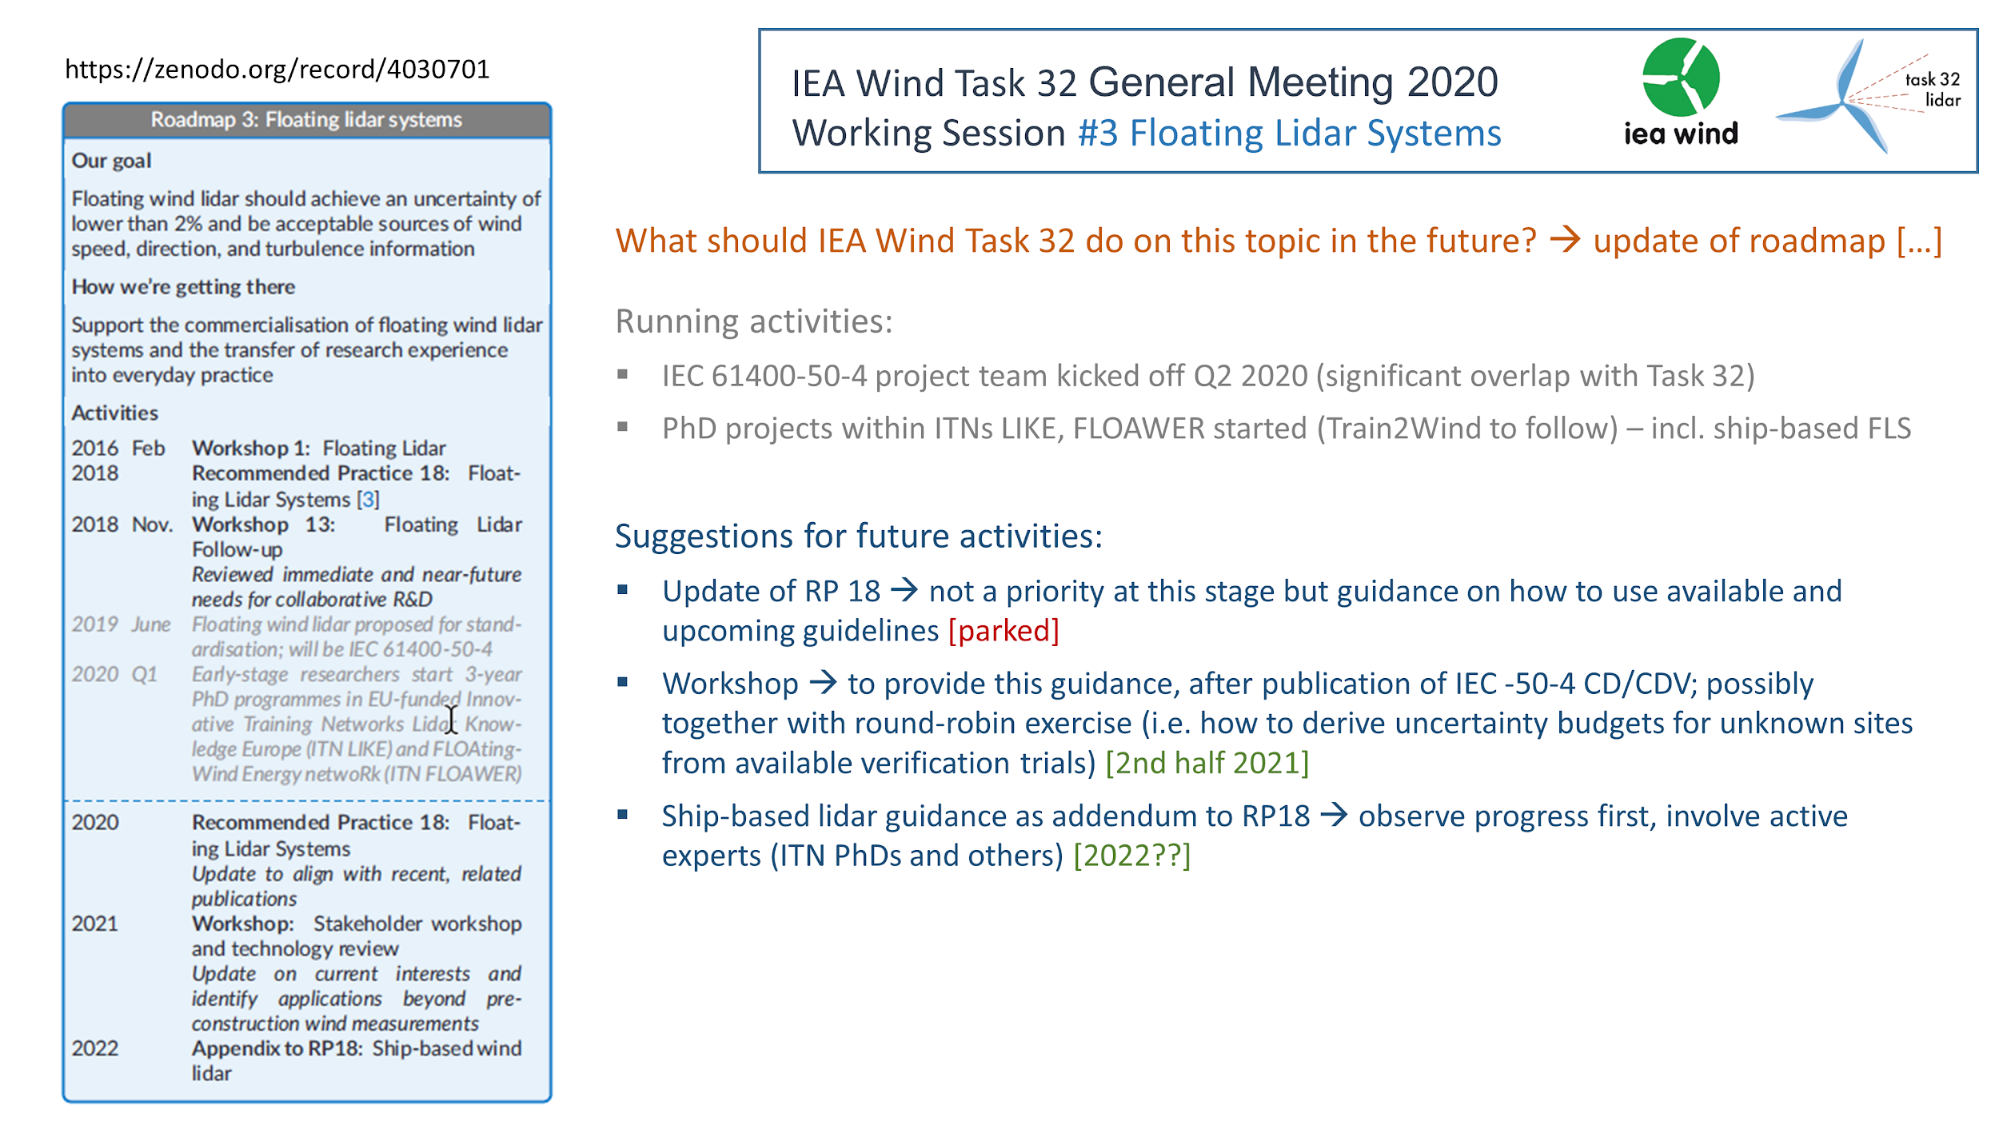
\includegraphics[width=0.85\textwidth]{figures/day3-floating-lidar.png}
%     }
%     \caption{Future activities for Task 32 around floating lidar systems.}
%     \label{fig:day3-floating-lidar}
% \end{figure*}

\begin{taskactions}
\textbf{Task 32 action}: Task 32 will organise an alignment workshop in
the second half of 2021.
\end{taskactions}

\subsubsection{Nacelle lidar in complex terrain}
\emph{Rapporteur: Jacob Burrows}

This group found that their biggest difficulty was in actually defining the problem. They produced a framework to help them and others think through the problem (\fref{fig:day3-nacelle-mounted}).

% \begin{figure*}[p]
%     \centering
%     \fbox{
%     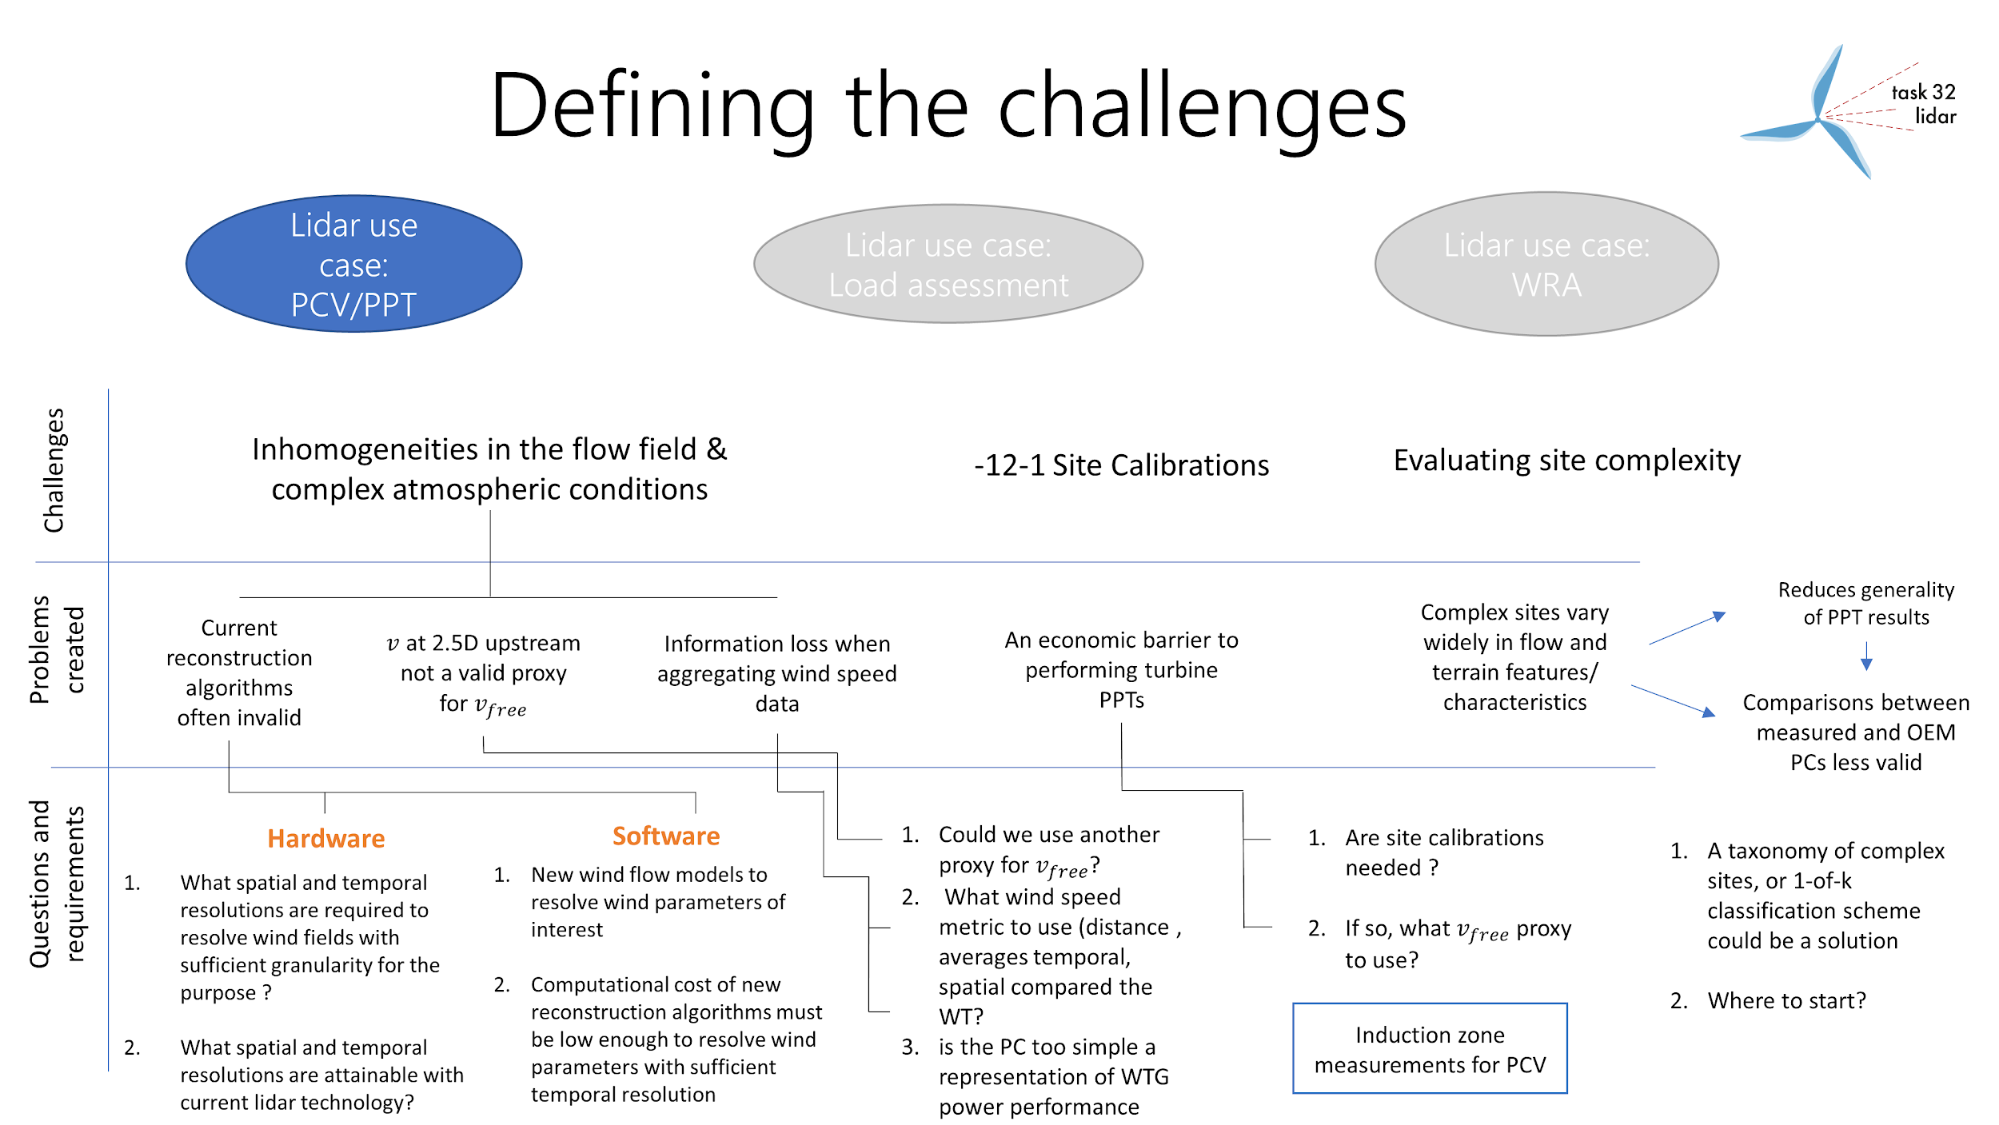
\includegraphics[width=0.85\textwidth]{figures/day3-nacelle-mounted.png}
%     }
%     \caption{Defining the challenge of using nacelle mounted lidar in complex terrain}
%     \label{fig:day3-nacelle-mounted}
% \end{figure*}

\begin{itemize}
    \item Comment from a participant: the 2.5$D$ is not a function of decay but a function of the turbine itself. Depends on the turbine size.
    \item The need is there to perform power curve verification in complex terrain from industry perspective
    \item There could be another workshop on this topic!
\end{itemize}

\begin{taskactions}
\textbf{Task 32 action}: Task 32 will combine the outcome from this group with the outcomes from the group looking at power performance verification using measurements in the induction zone. We'll also combine this with previous plans to run a round-robin on this theme. We'll propose a path forward in 2021.
\end{taskactions}

\subsubsection{Power performance verification in the induction zone}

\emph{Rapporteur: Sebastian Streitz}

The need for an alternative proxy for freestream wind speed is in common with nacelle lidar (\fref{fig:day3-powerperformance}). This suggests a need for more studies, and could also be topic for a short focused meeting.

% \begin{figure*}[p]
%     \centering
%     \fbox{
%     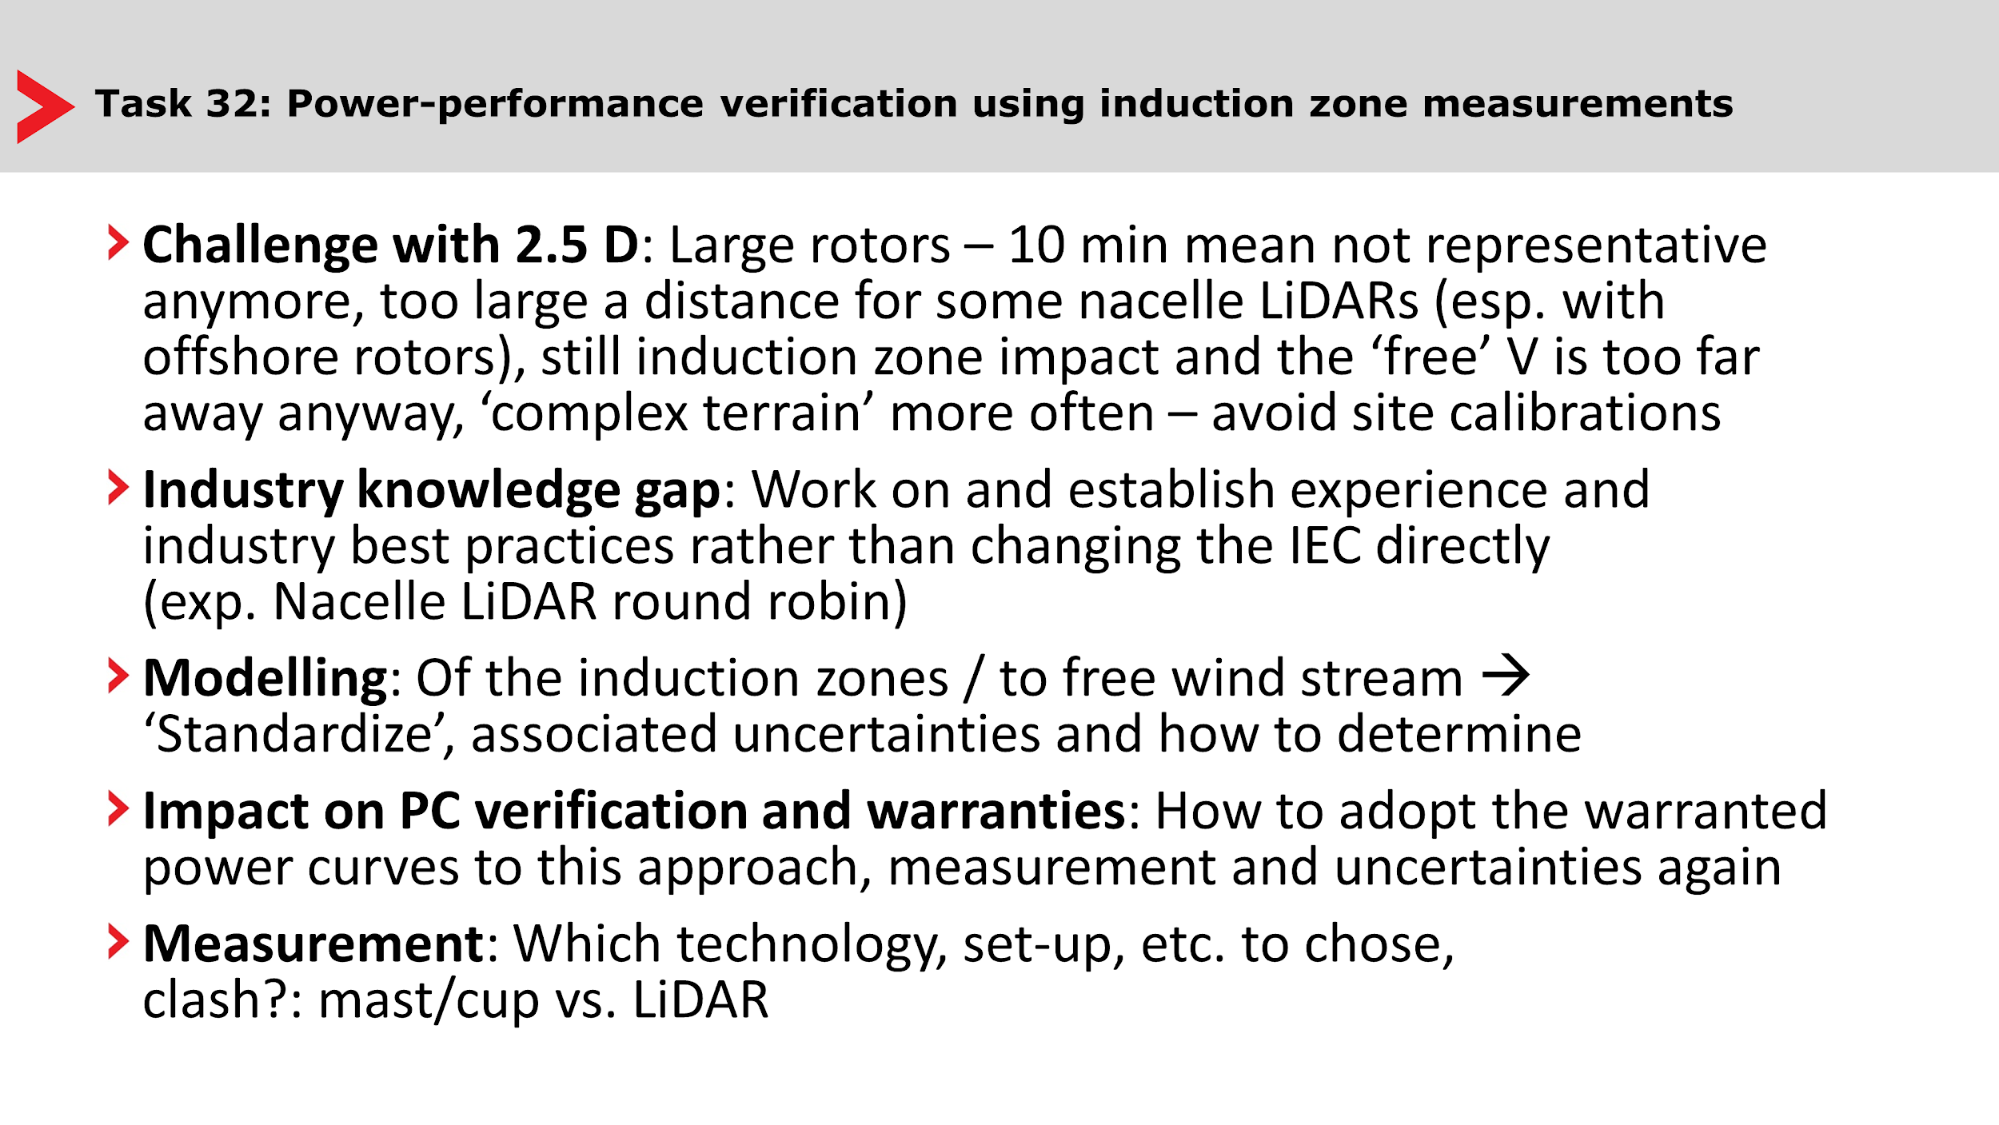
\includegraphics[width=0.85\textwidth]{figures/day3-powerperformance.png}
%     }
%     \caption{Opportunities and challenges with using measurements in the induction zone for power performance testing}
%     \label{fig:day3-powerperformance}
% \end{figure*}

\begin{taskactions}
\textbf{Task 32 action}: Task 32 will combine the outcome from this group with the outcomes from the group looking at nacelle mounted lidar in complex terrain. We'll also combine this with previous plans to run a round-robin on this theme. We'll propose a path forward in 2021.
\end{taskactions}

\subsubsection{Lidar-assisted control}

Lidar-assisted control of wind turbines is increasingly becoming reality, but turbines are not yet being designed to take full advantage of the wind lidar. There are still steps that need to be taken before co-design will become practical.

\begin{taskactions}
\textbf{Task 32 action}: Task 32 will:
\begin{enumerate}
\item Continue to work on a open repository of lidar-assisted control simulations
\item Address the cost of the lidar by a white paper: show that it has come down, improve lidar cost modeling
\item Organize a white paper to connect turbine OEM's needs to lidar manufacturers, e.g. improved availability, maintenance friendly, more adjustable
\item Collaborate more with other IEA Wind Tasks, for example Task 37 \& the new wind farm flow control Task.
\end{enumerate}
\end{taskactions}

% \begin{figure*}[p]
%     \centering
%     \fbox{
%     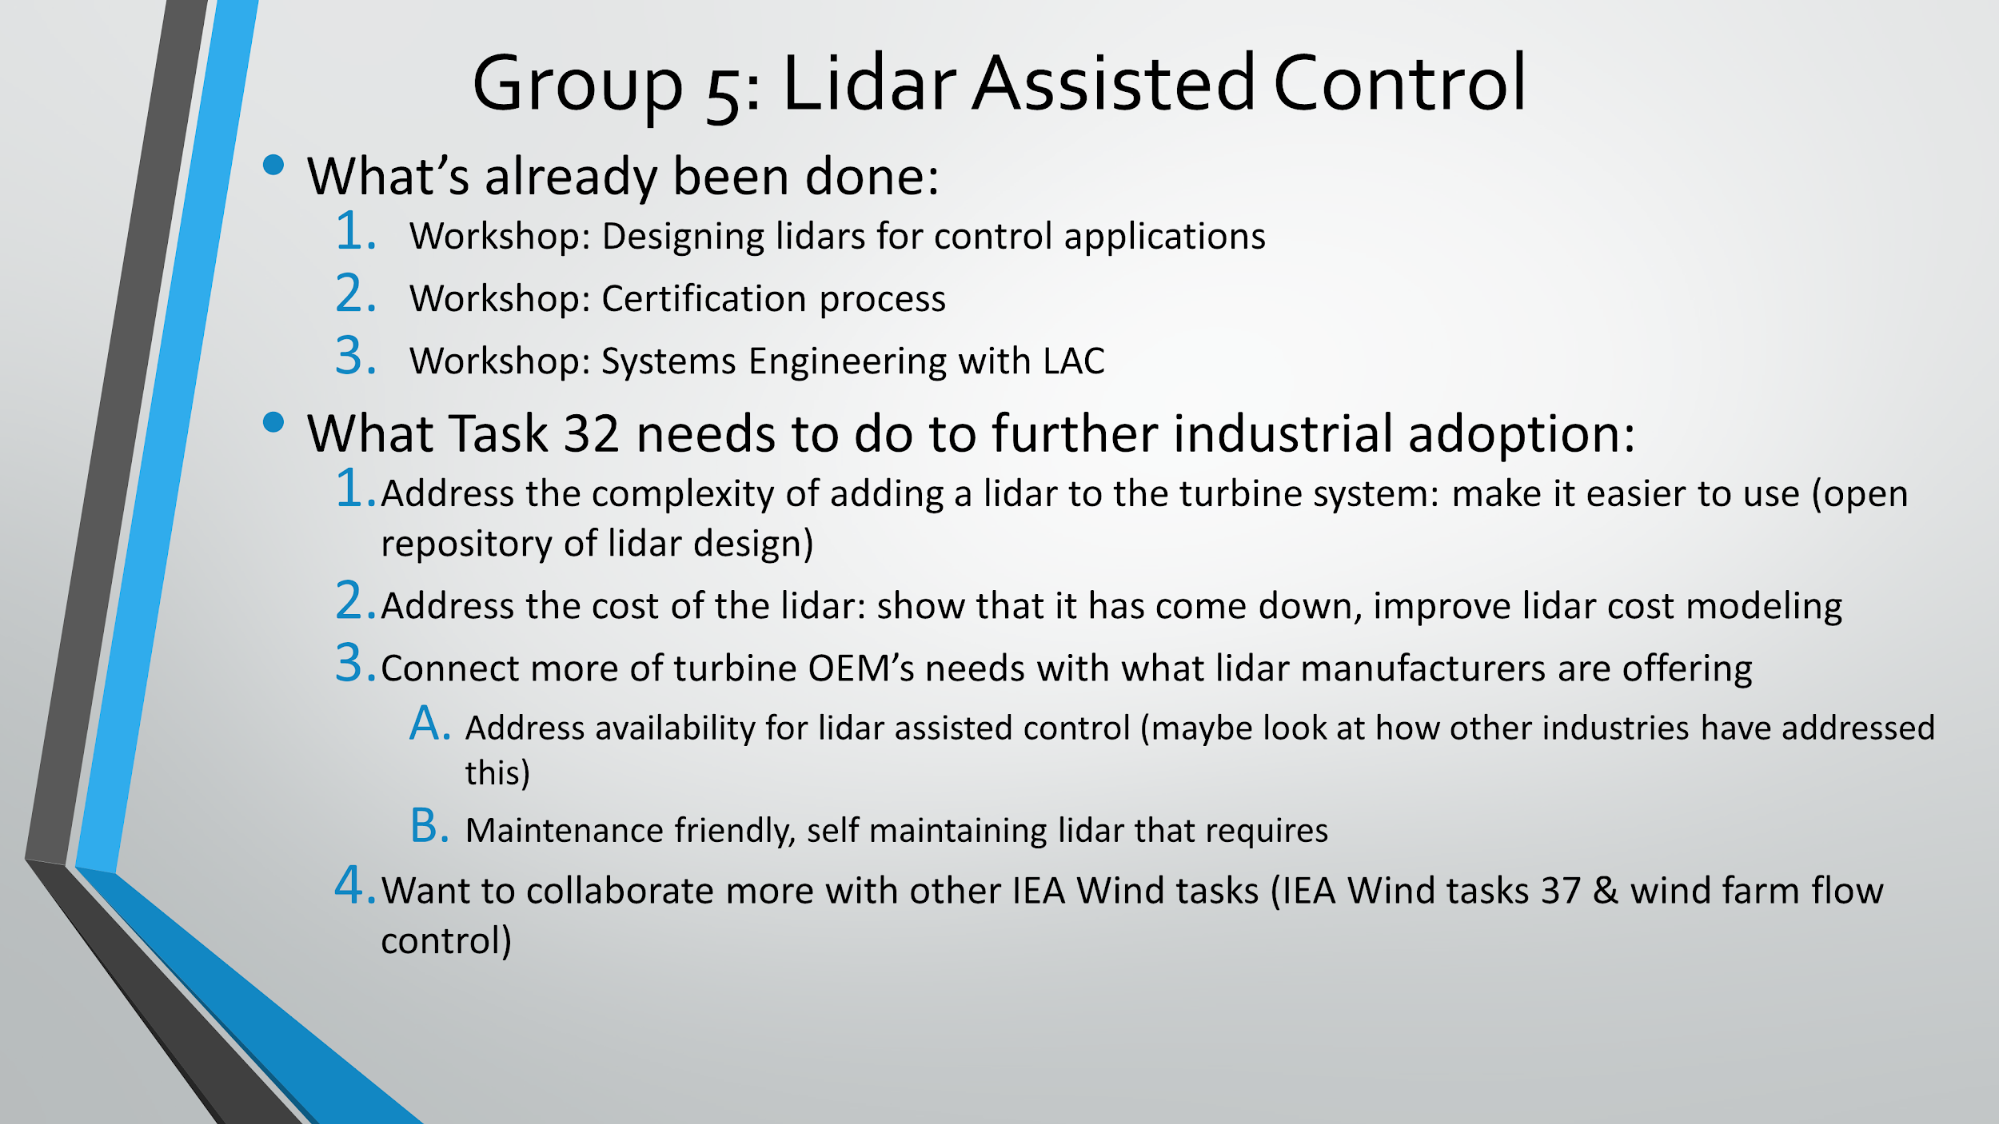
\includegraphics[width=0.85\textwidth]{figures/day3-LAC.png}
%     }
%     \caption{How Task 32 can enable adoption of lidar-assisted control of wind turbines and plants}
%     \label{fig:day3-LAC}
% \end{figure*}

The meeting closed at 17:00 CEST on 22 October.
